\documentclass[tikz,border=9pt]{standalone}
\usepackage[T1]{fontenc}
\usepackage{newtxtext,newtxmath}
\usepackage{tikz}
\usetikzlibrary{arrows.meta,positioning,fit,calc,backgrounds}

\begin{document}
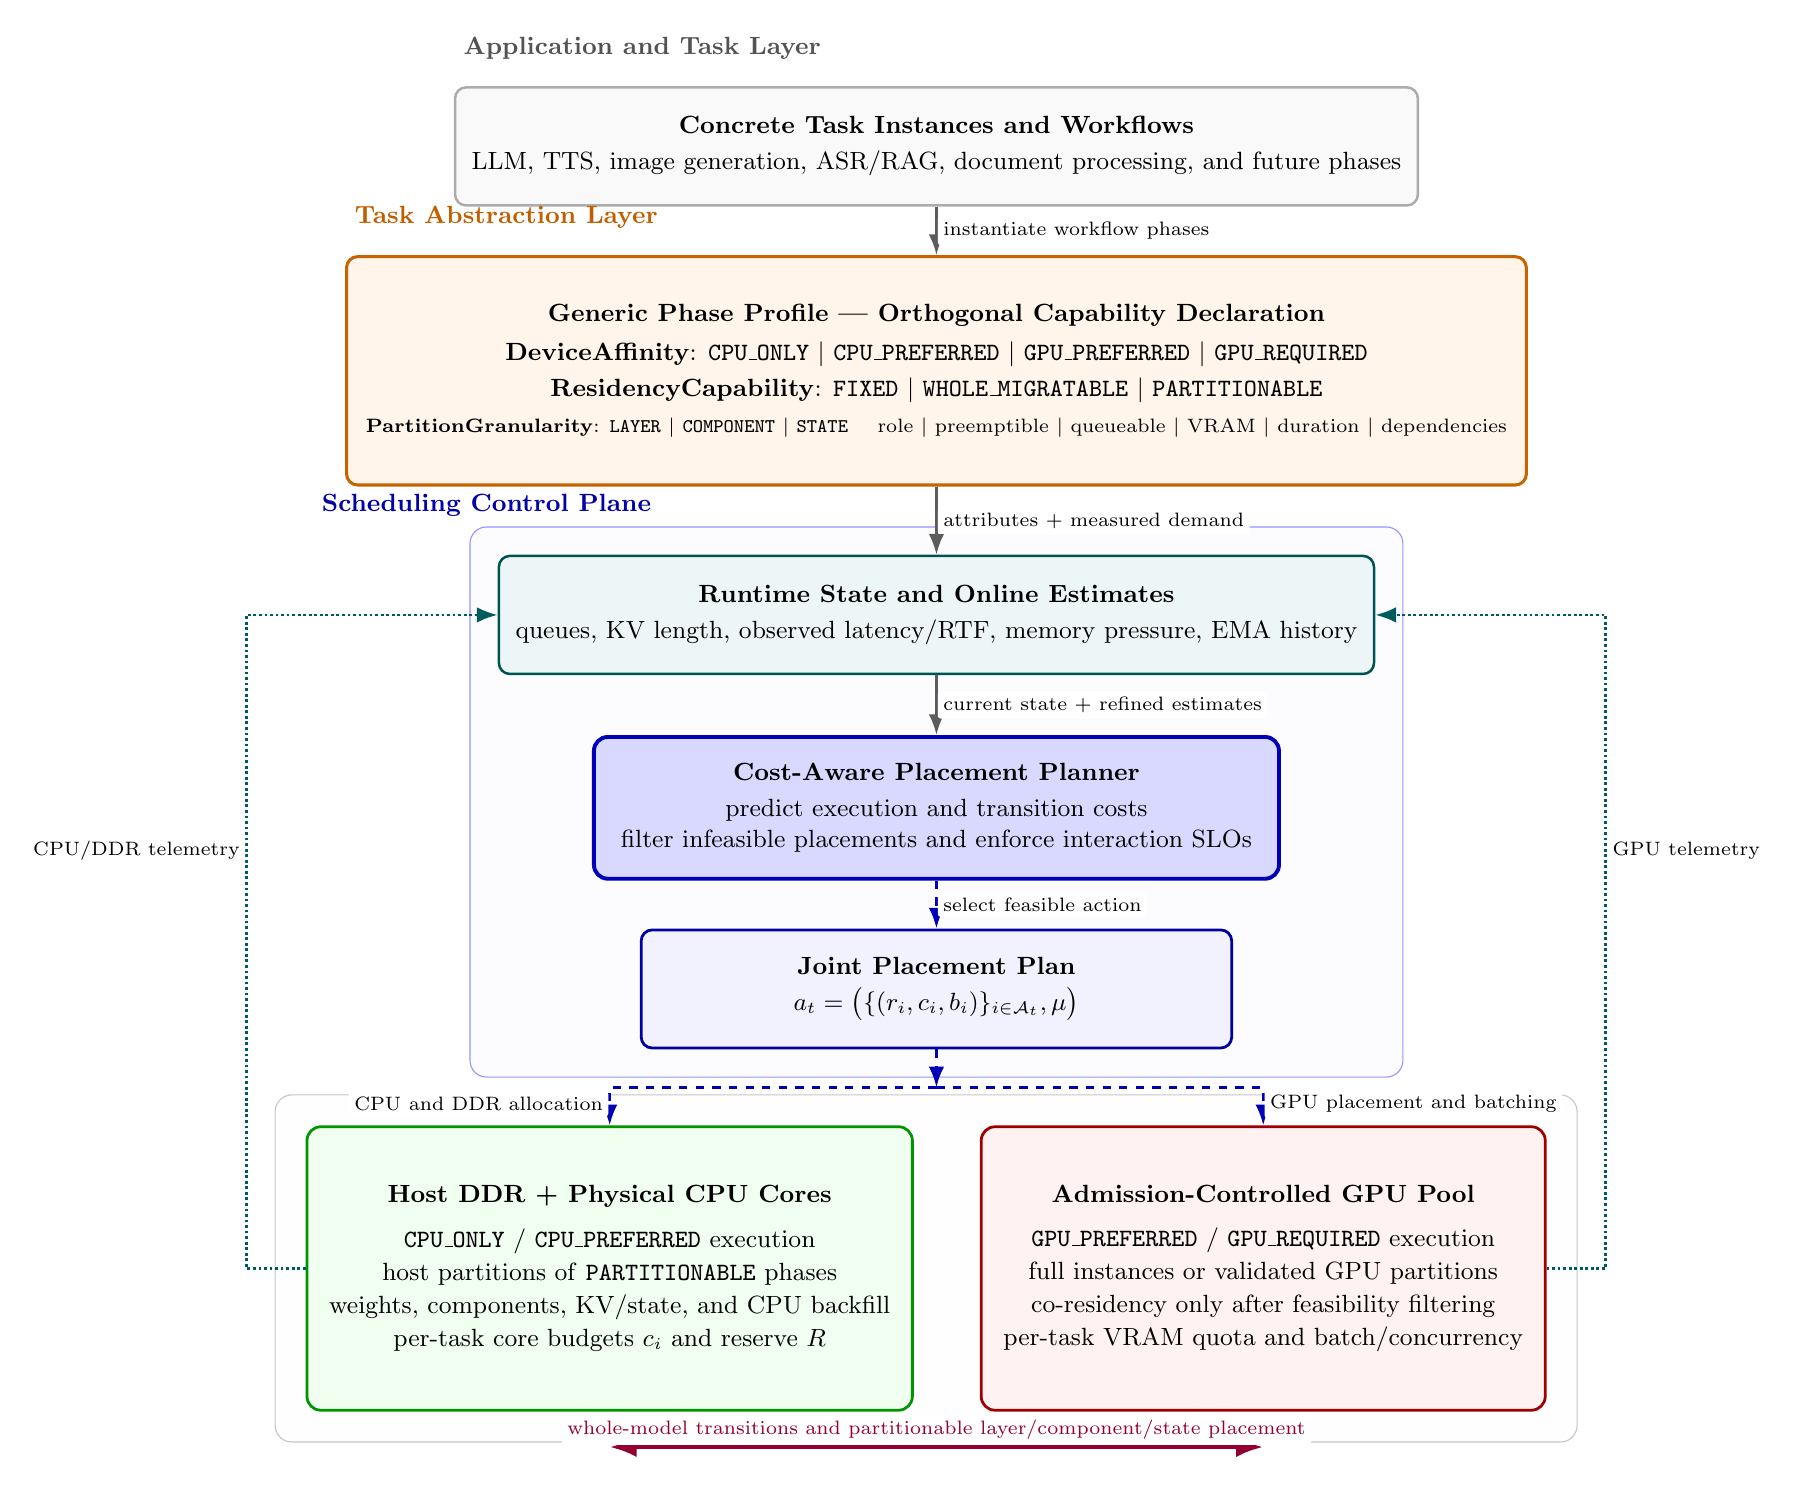
\begin{tikzpicture}[
    >=Latex,
    font=\small,
    workload/.style={
        draw=gray!65,
        fill=gray!5,
        rounded corners=4pt,
        line width=0.9pt,
        minimum width=122mm,
        minimum height=15mm,
        align=center,
        inner sep=6pt
    },
    profile/.style={
        draw=orange!78!black,
        fill=orange!8,
        rounded corners=4pt,
        line width=1.1pt,
        minimum width=122mm,
        minimum height=29mm,
        align=center,
        inner sep=7pt
    },
    state/.style={
        draw=teal!65!black,
        fill=teal!7,
        rounded corners=4pt,
        line width=0.9pt,
        minimum width=87mm,
        minimum height=15mm,
        align=center,
        inner sep=6pt
    },
    planner/.style={
        draw=blue!72!black,
        fill=blue!15,
        rounded corners=5pt,
        line width=1.4pt,
        minimum width=87mm,
        minimum height=18mm,
        align=center,
        inner sep=7pt
    },
    plan/.style={
        draw=blue!62!black,
        fill=blue!5,
        rounded corners=4pt,
        line width=1.0pt,
        minimum width=75mm,
        minimum height=15mm,
        align=center,
        inner sep=6pt
    },
    hostpool/.style={
        draw=green!58!black,
        fill=green!6,
        rounded corners=5pt,
        line width=1.0pt,
        minimum width=64mm,
        minimum height=36mm,
        align=center,
        inner sep=8pt
    },
    gpupool/.style={
        draw=red!62!black,
        fill=red!5,
        rounded corners=5pt,
        line width=1.0pt,
        minimum width=64mm,
        minimum height=36mm,
        align=center,
        inner sep=8pt
    },
    dataflow/.style={
        ->,
        draw=gray!72!black,
        line width=1.0pt
    },
    control/.style={
        ->,
        draw=blue!72!black,
        dashed,
        line width=1.0pt
    },
    feedback/.style={
        ->,
        draw=teal!72!black,
        densely dotted,
        line width=1.0pt
    },
    migration/.style={
        <->,
        draw=purple!78!black,
        line width=1.5pt
    },
    edgelabel/.style={
        fill=white,
        rounded corners=1pt,
        inner sep=2pt,
        align=center,
        font=\scriptsize
    }
]

% ------------------------------------------------------------------
% Application layer
% ------------------------------------------------------------------
\node[workload] (workload) at (0,11.1) {
    \textbf{Concrete Task Instances and Workflows}\\[2pt]
    {\small LLM, TTS, image generation, ASR/RAG, document processing, and future phases}
};

\node[font=\small\bfseries,text=gray!65!black,anchor=south west]
    at ($(workload.north west)+(0,0.22)$) {Application and Task Layer};

% Tasks are never routed by model name. Each phase is first mapped to the
% common attribute space consumed by both the Python and C++ schedulers.
\node[profile] (profile) at (0,8.25) {
    \textbf{Generic Phase Profile --- Orthogonal Capability Declaration}\\[3pt]
    {\small \textbf{DeviceAffinity}: \texttt{CPU\_ONLY} $\mid$
    \texttt{CPU\_PREFERRED} $\mid$ \texttt{GPU\_PREFERRED} $\mid$
    \texttt{GPU\_REQUIRED}}\\[2pt]
    {\small \textbf{ResidencyCapability}: \texttt{FIXED} $\mid$
    \texttt{WHOLE\_MIGRATABLE} $\mid$ \texttt{PARTITIONABLE}}\\[2pt]
    {\scriptsize \textbf{PartitionGranularity}: \texttt{LAYER} $\mid$
    \texttt{COMPONENT} $\mid$ \texttt{STATE} \quad
    role $\mid$ preemptible $\mid$ queueable $\mid$ VRAM $\mid$ duration $\mid$ dependencies}
};

\node[font=\small\bfseries,text=orange!75!black,anchor=south west]
    at ($(profile.north west)+(0,0.22)$) {Task Abstraction Layer};

% ------------------------------------------------------------------
% Control plane: one vertical decision path
% ------------------------------------------------------------------
\node[state] (state) at (0,5.15) {
    \textbf{Runtime State and Online Estimates}\\[2pt]
    {\small queues, KV length, observed latency/RTF, memory pressure, EMA history}
};

\node[planner] (planner) at (0,2.7) {
    \textbf{Cost-Aware Placement Planner}\\[2pt]
    {\small predict execution and transition costs}\\
    {\small filter infeasible placements and enforce interaction SLOs}
};

\node[plan] (plan) at (0,0.4) {
    \textbf{Joint Placement Plan}\\[2pt]
    {$a_t=\bigl(\{(r_i,c_i,b_i)\}_{i\in\mathcal A_t},\mu\bigr)$}
};

\draw[dataflow] (workload) --
    node[edgelabel,right] {instantiate workflow phases} (profile);
\draw[dataflow] (profile) --
    node[edgelabel,right] {attributes + measured demand} (state);
\draw[dataflow] (state) --
    node[edgelabel,right] {current state + refined estimates} (planner);
\draw[control] (planner) --
    node[edgelabel,right] {select feasible action} (plan);

\begin{pgfonlayer}{background}
    \node[
        draw=blue!42,
        fill=blue!1,
        rounded corners=6pt,
        inner sep=10pt,
        fit=(state)(planner)(plan),
        label={[font=\small\bfseries,text=blue!65!black]above left:Scheduling Control Plane}
    ] (controlbg) {};
\end{pgfonlayer}

% ------------------------------------------------------------------
% Heterogeneous resource plane
% ------------------------------------------------------------------
\node[hostpool] (host) at (-4.15,-3.15) {
    \textbf{Host DDR + Physical CPU Cores}\\[5pt]
    \texttt{CPU\_ONLY} / \texttt{CPU\_PREFERRED} execution\\[1pt]
    host partitions of \texttt{PARTITIONABLE} phases\\[1pt]
    weights, components, KV/state, and CPU backfill\\[1pt]
    {\small per-task core budgets $c_i$ and reserve $R$}
};

\node[gpupool] (gpu) at (4.15,-3.15) {
    \textbf{Admission-Controlled GPU Pool}\\[5pt]
    \texttt{GPU\_PREFERRED} / \texttt{GPU\_REQUIRED} execution\\[1pt]
    full instances or validated GPU partitions\\[1pt]
    co-residency only after feasibility filtering\\[1pt]
    {\small per-task VRAM quota and batch/concurrency}
};

\coordinate (branch) at (0,-0.85);
\draw[control] (plan) -- (branch);
\draw[control] (branch) -|
    node[edgelabel,pos=0.72,left] {CPU and DDR allocation} (host.north);
\draw[control] (branch) -|
    node[edgelabel,pos=0.72,right] {GPU placement and batching} (gpu.north);

% Resource movement is deliberately separated from the control arrows so the
% mechanism remains visually dominant and easy to explain in the paper.
\draw[migration] ($(host.south)+(0,-0.45)$) --
    node[edgelabel,above,text=purple!78!black]
        {whole-model transitions and partitionable layer/component/state placement}
    ($(gpu.south)+(0,-0.45)$);

% Runtime feedback closes the loop on the outside of the figure.
\draw[feedback] (host.west) -- ++(-0.75,0) |-
    node[edgelabel,pos=0.32,left] {CPU/DDR telemetry} (state.west);
\draw[feedback] (gpu.east) -- ++(0.75,0) |-
    node[edgelabel,pos=0.32,right] {GPU telemetry} (state.east);

\begin{pgfonlayer}{background}
    \node[
        draw=gray!45,
        fill=gray!1,
        rounded corners=6pt,
        inner sep=11pt,
        fit=(host)(gpu)
    ] {};
\end{pgfonlayer}

\end{tikzpicture}
\end{document}
